\documentclass{article}

\usepackage[margin=0.5in,bottom=1in,footnotesep=1in]{geometry}

\usepackage{amsmath}


\usepackage{multicol}
\setlength{\columnsep}{1cm}
\usepackage[]{algorithm2e}

\usepackage{lipsum}% for dummy text
\usepackage[varg]{txfonts}
\usepackage{graphicx}
\usepackage{subcaption}
\usepackage{multirow}

\usepackage[font=small,labelfont={sf,bf}]{caption}


\usepackage{titlesec}
\titleformat{\section}{\fontfamily{phv}\fontsize{12}{15}\bfseries}{\thesection}{1em}{}
\titleformat{\subsection}{\fontfamily{phv}\fontsize{10}{15}\itshape}{\thesubsection}{1em}{}

\title{\textbf{FYS4150 Project 2: \\Schr\"odinger's equation for two electrons \\in a 3-dimensional harmonic oscillator well}}
\author{Marie Foss, Maria Hammerstr{{\o}}m}
\date{} % removes date from title

\begin{document}

\maketitle

\begin{abstract}
	\noindent \lipsum[1]
	\vspace*{2ex}
	
	\noindent \textbf{Github:} \textit{https://github.com/mariahammerstrom/Project2}
	\vspace*{2ex}
\end{abstract}



\begin{multicols}{2}

\section{Introduction}
The aim of this project is to solve Schr\"odinger's equation for two electrons in a three-dimensional harmonic oscillator well with and without a repulsive Coulomb interaction. We are first interested in the solution of the radial part of Schr\"odinger's equation for \textit{one} electron. This equation reads

\begin{equation*}\label{eq:schrod_radial}
	-\frac{\hbar^2}{2 m} \left ( \frac{1}{r^2} \frac{d}{dr} r^2 \frac{d}{dr} - \frac{l (l + 1)}{r^2} \right )R(r) + V(r) R(r) = E R(r).
\end{equation*}
In our case $V(r)$ is the harmonic oscillator potential $(1/2)kr^2$ with $k=m\omega^2$ and $E$ is the energy of the harmonic oscillator in three dimensions. The quantum number $l$ is the orbital momentum of the electron. The oscillator frequency is $\omega$ and the energies are

\begin{equation*}
	E_{nl}=  \hbar \omega \left(2n+l+\frac{3}{2}\right),
\end{equation*}
with $n=0,1,2,\dots$ and $l=0,1,2,\dots$. In this project we use $l = 0$. 

We will solve Eq. (\ref{eq:schrod_radial}) by reformulating it in a discretized form as an eigenvalue equation to be solved with Jacobi's method. 

After some substitutions and introducing the dimensionless variable $\rho = (1/ \alpha) r$ where $\alpha$ is of dimension length, we can rewrite Eq. (\ref{eq:schrod_radial}) as

\begin{equation*}
	-\frac{d^2}{d\rho^2} u(\rho) + \rho^2u(\rho)  = \lambda u(\rho) .
\end{equation*}
This is the first equation to solve numerically. In three dimensions the eigenvalues for $l=0$ are $\lambda_0=3,\lambda_1=7,\lambda_2=11,\dots .$

We use the by now standard expression for the second derivative of a function $u$

\begin{equation*}\label{eq:diffoperation}
    u''=\frac{u(\rho+h) -2u(\rho) +u(\rho-h)}{h^2} +O(h^2),
\end{equation*} 
where $h$ is our step length. For a given number of steps $n_{\mathrm{step}}$, the step length is defined as

\begin{equation}
	  h=\frac{\rho_{\mathrm{max}}-\rho_{\mathrm{min}} }{n_{\mathrm{step}}}.
\end{equation}
Next we define minimum and maximum values for the variable $\rho$, $\rho_{\mathrm{min}}=0$  and $\rho_{\mathrm{max}}$, respectively. Define an arbitrary value of $\rho$ as 

\begin{equation}
	\rho_i= \rho_{\mathrm{min}} + ih \hspace{1cm} i=0,1,2,\dots , n_{\mathrm{step}}.
\end{equation}
Now we can write the Schr\"odinger equation in a compact way

\begin{equation*}
	-\frac{u_{i+1} -2u_i +u_{i-1}}{h^2}+\rho_i^2u_i=-\frac{u_{i+1} -2u_i +u_{i-1} }{h^2}+V_iu_i  = \lambda u_i,
\end{equation*}
where $V_i=\rho_i^2$ is the harmonic oscillator potential.

Define first the diagonal matrix element

\begin{equation}
   d_i=\frac{2}{h^2}+V_i,
\end{equation}
and the non-diagonal matrix element (which is a mere constant, and are all equal) 

\begin{equation}
   e_i=-\frac{1}{h^2}.
\end{equation}
With these definitions the Schr\"odinger equation takes the following form

\begin{equation}
d_iu_i+e_{i-1}u_{i-1}+e_{i+1}u_{i+1}  = \lambda u_i,
\end{equation}
where $u_i$ is unknown. We can write the latter equation as a matrix eigenvalue problem 

\begin{equation}\label{eq:sematrix}
    \left( \begin{array}{cccccc} 		
    d_1	& e_1	& 0		& \dots & 0	& 0 \\
	e_1 & d_2 	& e_2  	& \dots	& 0 & 0 \\
	0	& e_2 	& d_3 	& e_3	&\dots 	& 0\\
	\dots & \dots & \dots &\dots &\dots & \dots\\
	0 	& \dots & \dots &\dots &d_{n_{\mathrm{step}}-2} 		& e_{n_{\mathrm{step}}-1}\\
	0   & \dots & \dots  &\dots &e_{n_{\mathrm{step}}-1} 		& d_{n_{\mathrm{step}}-1}

    \end{array} \right)
    \left( \begin{array}{c} u_{1} \\ u_{2} \\ \dots\\ \dots\\ \dots \\ u_{n_{\mathrm{step}}-1} \end{array} \right)
    = \lambda \left( \begin{array}{c} u_{1} \\ u_{2} \\ \dots\\
    \dots\\ \dots\\ u_{n_{\mathrm{step}}-1} \end{array} \right) 
\end{equation} 
Secondly, we will consider the Schr\"odinger equation for \textit{two} electrons by studying two electrons in a harmonic oscillator well which also interact via a repulsive Coulomb interaction.

We start by writing the single-electron equation as

\begin{equation*}
	-\frac{\hbar^2}{2 m} \frac{d^2}{dr^2} u(r) + \frac{1}{2}k r^2u(r)  = E^{(1)} u(r),
\end{equation*}
where $E^{(1)}$ stands for the energy with one electron only. For two electrons with \textit{no} repulsive Coulomb interaction, we have the following Schr\"odinger equation:

\begin{equation*}
	\left(  -\frac{\hbar^2}{2 m} \frac{d^2}{dr_1^2} -\frac{\hbar^2}{2 m} \frac{d^2}{dr_2^2}+ \frac{1}{2}k r_1^2+ \frac{1}{2}k r_2^2\right)u(r_1,r_2)  = E^{(2)} u(r_1,r_2) .
\end{equation*}
After a series of substitutions, this can be written as

\begin{equation}\label{eq:coulomb}
	- \frac{d^2}{d \rho^2} \psi (\rho) + \omega_r^2 \rho^2 \psi (\rho) + \frac{1}{\rho}  = \lambda \psi (\rho)
\end{equation}
In this case the potential is:

\begin{equation}
	V_i = \omega_r^2 \rho^2 + 1/\rho
\end{equation}
where we will study the cases where the oscillator frequency $\omega_r$ is $\omega_r = 0.01$, $\omega_r = 0.5$, $\omega_r = 1$ and $\omega_r = 5$ for the ground state only, that is, the lowest-lying state. 



\section{Methods}
\subsection{Jacobi's method}
In this project we will use Jacobi's method to find the eigenvalues, which consists of doing a number of similarity transformations

\begin{equation*}
	\textbf{S}^T \textbf{AS} = \textbf{B}
\end{equation*}
where \textbf{A} is the matrix in our given problem, and \textbf{S} is an $(n \times n)$ orthogonal transformation matrix

\begin{equation*}
	\textbf{S} = \left( \begin{array}{cccccccc} 
				1 		& 0 		& \dots    		& 0    					& 0  		&\dots      	& 0 		& 0 \\
                                	0 		& 1 		& \dots  		& 0    					& 0  		&\dots     	& 0		& 0 \\
                                	\dots  	& \dots 	& \dots 		& \dots  					&\dots      	&\dots 	& 0		& \dots \\
                                	0   		& 0 		& \dots 		& \textrm{cos } \theta 		&0       	& \dots	& 0		& \textrm{sin } \theta \\
				0 		& 0 		& \dots  		& 0    					& 1  		&\dots     	& 0		& 0 \\
				\dots 	& \dots 	& \dots  		& \dots    					& \dots  	&\dots     	& 0		& \dots \\
				0 		& 0 		& \dots  		& 0    					& 0  		&\dots     	& 1		& 0 \\
				0 		& 0 		& \dots  		& - \textrm{sin } \theta  		& \dots  	&\dots     	& 0		& \textrm{cos } \theta


             \end{array} \right).
\end{equation*} 
The recipe is to choose $\theta$ so that all non-diagonal matrix elements $b_{kl}$ become zero. 

In the algorithm we define the quantities tan $\theta = t = s/c$ with $s$ = sin $\theta$ and $c$ = cos $\theta$. By some manipulations, we can write:

\begin{equation}\label{eq:cos}
	c = \frac{1}{\sqrt{1+t^2}}.
\end{equation}
This is used to calculate the difference between matrices \textbf{B} and \textbf{A}, which we want to minimize:

\begin{equation}
	||{\bf B}-{\bf A}||_F^2=4(1-c)\sum_{i=1,i\ne k,l}^n(a_{ik}^2+a_{il}^2) +\frac{2a_{kl}^2}{c^2}.
\end{equation}
In order to minimize this equation, $c$ should be as close to 1 as possible. Making $t$ as small as possible, will create this effect, as seen in Eq. (\ref{eq:cos}).

The \textbf{algorithm} can be described as follows: 

\begin{itemize}
	\item Choose a tolerance $\epsilon$, typically $10^{-8}$ or smaller.
	\item Find matrix element $a_{kl}$ with the largest value and its indices $k$ and $l$.
	\item Check that max$(a_{kl}^2) > \epsilon$ for the off-diagonal matrix elements.
	\item Compute $\tau$, sin $\theta$, cos $\theta$, tan $\theta$.
	\item Compute the similarity transformations for this set of values for $(k,l)$, which will create a new matrix, \textbf{B} = \textbf{S}$(k,l,\theta)^T$\textbf{A}\textbf{S}$(k,l,\theta)$.
	\item Continue to follow these steps until max$(a_{kl}^2) > \epsilon$ is no longer the case.
\end{itemize}

\subsection{Numerical library}
In addition to solving the problem in a brute-force way using Jacobi's method, we have also used the numerical library Armadillo, and compared the results from these two methods.



\section{Results}
\subsection{Harmonic oscillator}
In the case of the harmonic oscillator there is an analytical solution to what the lowest eigenvalues should be. For $l = 0$ these are $\lambda_0 = 3, \lambda_1 = 7, \lambda_2 = 11, \dots$ Solving this numerically will not lead to the exact values, but we can get very close to this. We have computed the eigenvalues using our algorithm as described in the previous section, as well as using the Armadillo package.

In order to get the lowest three eigenvalues with four leading digits, we need around $n_{\textrm{step}} = 200$. Then the lowest three eigenvalues are: $\lambda_0 = 2.999, \lambda_1 = 6.99$ and $\lambda_2 = 10.99$ using $\rho_{\textrm{max}} = 10.0$. 

The eigenvalues will depend on our choice for $\rho_{\textrm{max}}$. By testing we find that a lower $\rho_{\textrm{max}}$ makes the eigenvalues is more precise for $\rho_{\textrm{max}} = 4.0$, but gets worse for lower values, making the eigenvalues larger than they should be. For values higher than 10.0 the eigenvalues also are bad, becoming too small.

The number of similarity transformation needed for the non-diagonal matrix elements to become zero depends on the dimensionality of the matrix. An upper limit to the allowed number of similarity transformations is in the range $12n^3 - 20n^3$. We have set the limit to $50n^3$ to be on the safe side. When running the code, the number of transformations is counted. For different dimensionalities we find (for $\rho_{\textrm{max}} = 10.0$):

\begin{center}
\begin{tabular}{ l l l}\hline
	$n$ 			& No. of iterations	 	& Time (s) \\ \hline
	5 			& 11 					& 0\\
	10 			& 41					& 0\\
	20 			& 176 				& 0\\
	50 			& 1727 				& 0\\
	100	  		& 11315				& 0 \\
	200  			& 61308				& 17 \\
	\hline
\end{tabular}
\end{center}
where the time is for our algorithm. Using Armadillo resulted in 0 seconds for all of the above $n$-values. Both methods give similar results for the eigenvalues. See \verb@selected_results.txt@ to see output examples.

We want to estimate the number of transformations and extract a behavior as function of the dimensionality of the matrix. The relationship between $n$ and number of iterations are plotted in Fig.~\ref{fig:iterations} where the blue line represents the output from our code and the red line is an approximation of $n^{2.1}$ we found to be a nice fit.

\begin{center}
	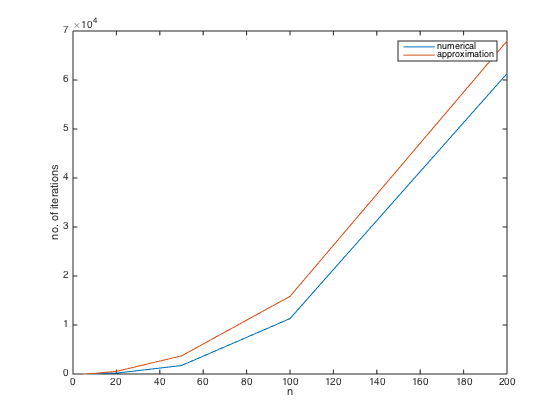
\includegraphics[width=90mm]{../build-Project2-Desktop_Qt_5_5_0_clang_64bit-Debug/iterations.png} 	
	\captionof{figure}{Number of iterations as a function of $n$, approximated by $n^{2.1}$ (blue).}
	\label{fig:iterations}
\end{center}
From comparisons with analytical solutions, we see that our program is working well and we can proceed with the next potential of interest.



\subsection{Harmonic oscillator with Coulomb interactions}
Next we want to study the harmonic oscillator with Coulomb interactions. For specific oscillator frequencies there is an analytical answer to Eq. (\ref{eq:coulomb}), described in the article by M. Taut, Phys. Rev. A 48, 3561 - 3566 (1993). Thus, we can compare our numerical solution with the analytical solution, given as:

\begin{equation}
\begin{aligned}
	V_0 &= \frac{3}{2} \bigg[ \frac{\omega_r}{2} \bigg]^{2/3} \\
	\omega_e &= \sqrt{3} \omega_r \\
	\epsilon_m^{'} &= V_0 + \omega_e [m + \frac{1}{2}] \textrm{,       } m = 0,1, \dots
\end{aligned}
\end{equation}
where $\epsilon_m^{'}$ gives the analytical eigenvalues.

For $n = 200$ and $\rho_{\textrm{max}} = 50.0$ we find:

\begin{center}
\begin{tabular}{ l l l l l }\hline
	$\omega_r$ 	& 0.01		& 0.5		& 1.0	&5.0\\ \hline
	$\lambda_0$ 	& 0.105773	& 2.22507		& 4.0372	& 16.9105\\
	$\lambda_1$ 	& 0.141504	& 4.11139		& 7.81445	& 34.4305 \\
	$\lambda_2$ 	& 0.178008	& 6.017		& 11.5845	& 49.9979\\
	\hline
\end{tabular}
\end{center}

\begin{center}
\begin{tabular}{ l l l l l }\hline
	$\omega_r$ 	& 0.01		& 0.5			& 1.0		&5.0\\ \hline
	$\epsilon_0^{'}$ 	& 0.0963808	& 1.62356		& 2.75591	& 9.85617\\
	$\epsilon_1^{'}$ 	& 0.113701	& 2.48959		& 4.48796	& 18.5164 \\
	$\epsilon_2^{'}$ 	& 0.131022	& 3.35561		& 6.22001	& 27.1767\\
	\hline
\end{tabular}
\end{center}
COMMENT!
%We see that the analytic and numerical eigenvalues correspond quite nicely for small $\omega_r$, but worsen for higher $\omega_r$ (stronger oscillator potential). According to the article we should have used a different expression for $\epsilon_m^{'}$ for large values of $\omega_r$. COMMENT.

We calculate the eigenvectors for the ground state using Armadillo's \verb@eigsym@ function. The eigenvectors represents the wave function. A plot of the wave function for two electrons as a function of relative coordinates $\rho$ and different values of $\omega_r$ is plotted in Fig.\ref{fig:wave_function}. We see that a stronger oscillator potential $\omega_r$ creates a deeper potential well, as expected. $\rho$ represents the distance between the two electrons, so we see that for a larger oscillator potential, the electrons will be closer.

For the case of $\omega_r = 0.01$, the chosen value of $\rho_{max}$ is important. $\rho_{max}$ needs to be quite large to make the plot come out right in this case. We landed on $\rho_{max} = 40$.

\begin{center}
	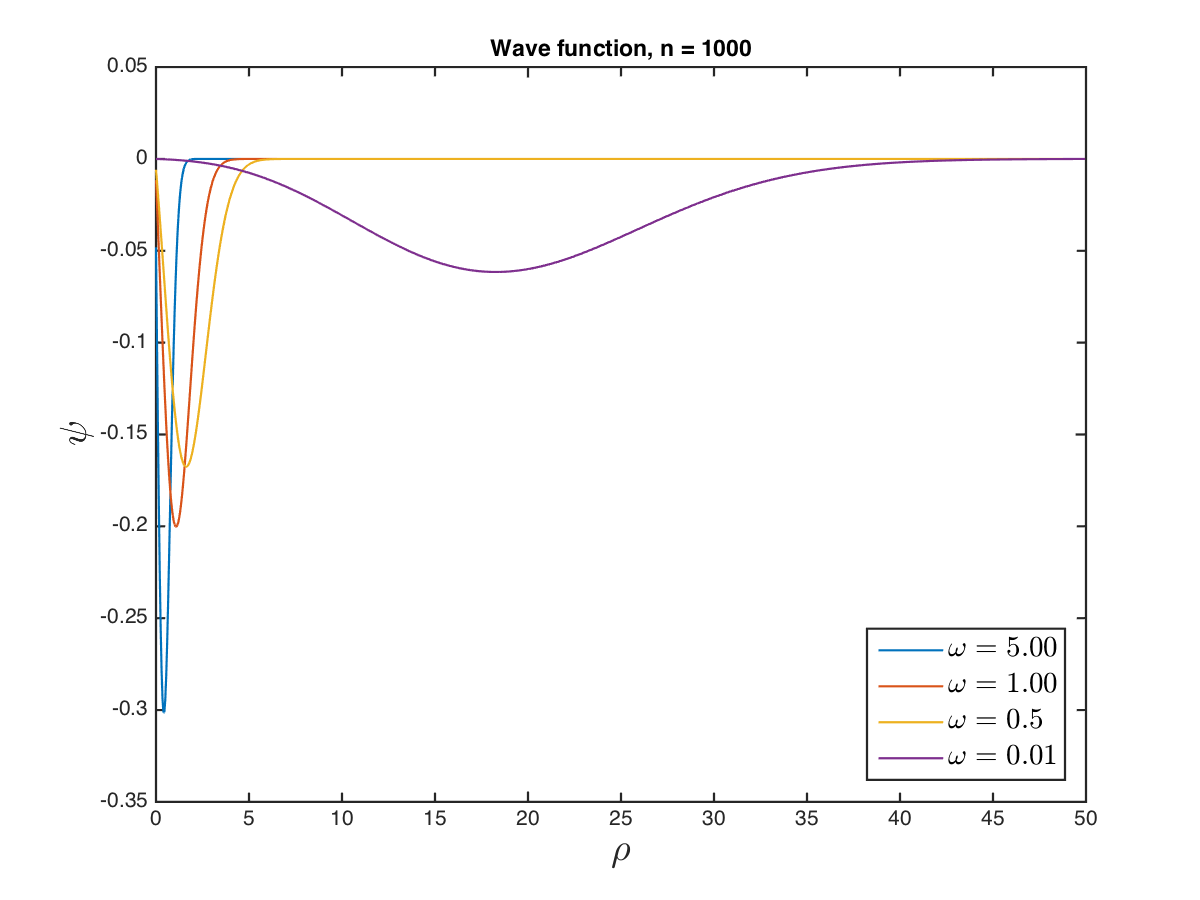
\includegraphics[width=90mm]{../build-Project2-Desktop_Qt_5_5_0_clang_64bit-Debug/wave_function.png} 	
	\captionof{figure}{The wave function.}
	\label{fig:wave_function}
\end{center}
By plotting the squared of the eigenvector values, we get the probability distribution, shown in Fig.~\ref{fig:prob_dist}. The figure shows the probability that the electrons will be in a given distance $\rho$.  COMMENT.

\begin{center}
	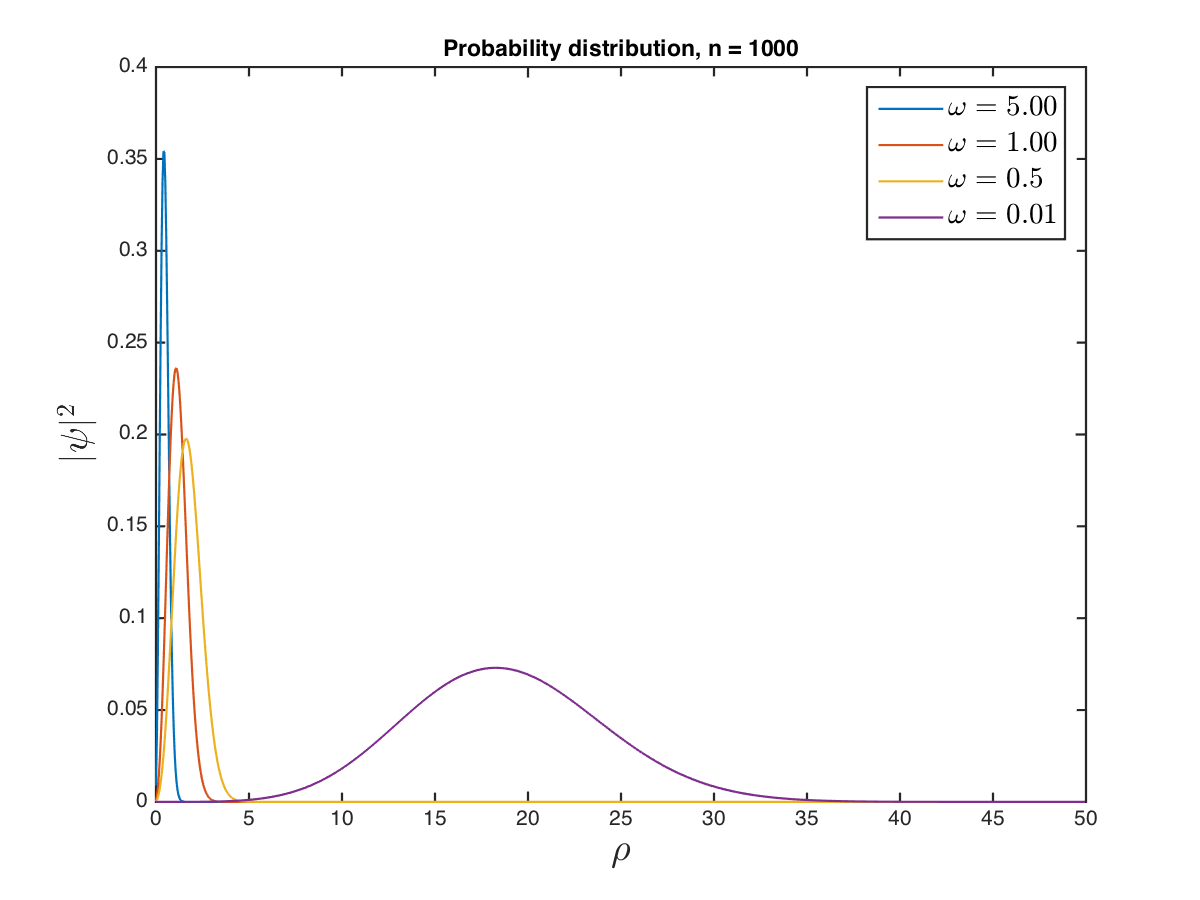
\includegraphics[width=90mm]{../build-Project2-Desktop_Qt_5_5_0_clang_64bit-Debug/probability_distribution.png} 	
	\captionof{figure}{The normalized probability distribution.}
	\label{fig:prob_dist}
\end{center}


\subsection{Unit tests}
In our code we have used several tests to make sure that the results are sound. The tests include:

\begin{itemize}
	\item Checking that the rotation matrix only makes one rotation when $n = 2$.
	\item Checking our results for the eigenvalues with analytical solutions.
\end{itemize}




\section{Conclusions}
...





\section{List of codes}

The codes developed for this project are:\\

\noindent \verb@main.cpp@ -- main program, C++

\noindent \verb@plotting.m@ -- plotting program, MATLAB

\end{multicols}

\end{document}
